\documentclass[10pt]{scrartcl}
\usepackage[T1]{fontenc}	% Passendes Fontencoding zur Suche im pdf
\usepackage{textcomp}		% das EUR-Zeichen für OT und T1
\usepackage{lmodern}
\usepackage[ngerman]{babel}	% neue deutsche Rechtschreibung
\usepackage[utf8]{inputenc}	% direkt deutsche Umlaute und EUR-Zeichen eingeben
\usepackage{graphicx,framed}	% Bilder, Rahmen
\usepackage{wrapfig}
\usepackage[a6paper,paperheight=21cm]{geometry}
\usepackage{fancyhdr}
\usepackage{url}
\usepackage{tikz}
\usepackage{draftwatermark}

\newcommand{\ffmagenta}{magenta}
\newcommand{\ffyellow}{yellow}
\newcommand{\fflogo}{
\draw (36mm,44mm) circle (22mm) [line width=1mm,color=\ffmagenta];
\draw (74mm,54mm) circle (22mm) [line width=1mm,color=\ffmagenta];
\draw (74mm,54mm) circle (29mm) [line width=6mm,color=\ffmagenta];
\fill[\ffyellow] (22mm,48mm) -- (22mm,52mm) -- (30mm,52mm) -- (26mm,56mm) -- (31mm,56mm) -- (37mm,50mm) -- (31mm,44mm) -- (26mm,44mm) -- (30mm,48mm);
\fill[\ffyellow] (64mm,50mm) -- (73mm,59mm) -- (81mm,59mm) -- (75mm,53mm) -- (88mm,53mm) -- (88mm,47mm) -- (75mm,47mm) -- (81mm,41mm) -- (73mm,41mm);
}

\SetWatermarkAngle{0}
\renewcommand{\ffmagenta}{magenta!25!white}
\renewcommand{\ffyellow}{yellow!25!white}
\SetWatermarkText{
\begin{tikzpicture}[scale=1.7,rotate=90]
\fflogo
\end{tikzpicture}
}

\pagestyle{fancy}
\fancyhead{
\begin{tikzpicture}
\draw (\topmargin,0) -- (\textwidth,0) [line width=5mm,color=yellow];
\node at (5.5,0) {freifunk rheinland e.V.};
\draw (0,-0.5) -- (\textwidth,-0.5) [line width=5mm,color=magenta];
\end{tikzpicture}
}
\fancyfoot{}
\renewcommand{\headrule}{}
\renewcommand{\footrule}{}

\setcounter{secnumdepth}{0}

\begin{document}
\section{\normalsize Was ist Freifunk?}
Freifunk ermöglicht jedem Bürger einen kostenfreien, unabhängigen Zugang zum Internet. Dieses Projekt wird von ehrenamtlichen Helfern aufgebaut und betreut. Das Ziel ist ein stadtweites, nichtkommerzielles Freifunknetz, welches man mittels einfacher \textbf{WLAN}-Technik nutzen kann. Gibt es genug Freifunk-Router in einer Gegend, verbinden sich die Geräte automatisch miteinander. Es entsteht ein großes Mesh-Netzwerk, eine \glqq Freifunkwolke\grqq, welche für alle \textbf{frei zugänglich} ist.

\section{\normalsize Warum sollte ich freifunken?}
Ist Dir bewusst, wie oft Du Dein Internet nicht benutzt? Teile einfach Dein Internet und lasse damit sozial benachteiligte Menschen, Besucher und frisch Zugezogene teilhaben und ermögliche ihnen den Zugang zu Wissen.

\section{\normalsize Ein Verein für Freifunk?}
\begin{wrapfigure}{R}{80px}

\includegraphics[scale=0.2]{Verein}
\end{wrapfigure}
Daher haben sich Freifunker aus vielen Städten NRWs zusammengeschlossen und diesen Verein ins Leben gerufen.
Unser Ziel ist es, den Freifunk in den Regionen des Rheinlands zu fördern und bekannter zu machen.
\textbf{Hilf uns dabei!}
\lfoot{\tiny v.i.S.d.P. freifunk rheinland e.V., Postfach 27 01 02, 40524 Düsseldorf}

\newpage
\lfoot{\footnotesize\url{www.freifunk-rheinland.net}\\\url{kontakt@freifunk-rheinland.net}\\\tiny\centering Konto 4 044 542 600, BLZ 430 609 67, GLS Gemeinschaftsbank eG}
\rfoot{\footnotesize\url{@ffrhein}\\02 11/41 74 12 21}

\section{\normalsize Die Ziele unseres Vereins}
Unter dem Dach eines gemeinnützigen Vereins fällt es uns leichter, an die Öffentlichkeit zu treten und Unterstützer zu finden. Wir bieten zudem unseren Mitgliedern Zugang zu Know-How, Infrastruktur und rechtlichen Schutz.

\section{\normalsize Du kannst uns helfen!}
\begin{wrapfigure}{R}{60px}
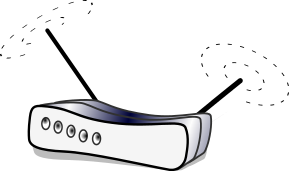
\includegraphics[scale=0.4]{Router}
\end{wrapfigure}
Werde Mitglied und unterstütze die Vereinsarbeit. Wir arbeiten ehrenamtlich, doch Router, Kabel und Antennen kosten Geld. Wir sind auf Spenden und Mitgliedsbeiträge angewiesen.

Hilf uns, neue Standorte für Freifunk-Router zu finden. Ideal ist, wenn sie hoch und zentral platziert sind. Kontakte zu Kirchen und Hausverwaltern/-besitzern sind sehr hilfreich. Stelle einen Freifunkrouter bei Dir auf, wir helfen Dir dabei!

Erzähle anderen von unserem Projekt!

\section{\normalsize Du möchtest uns persönlich kennenlernen?}
Komm einfach zu einem unserer Treffen oder nimm Kontakt zu uns auf:
\end{document}
